\documentclass[11pt,a4paper]{article}

% __Paquetes__

%\renewcommand{\familydefault}{\sfdefault}
\usepackage[spanish]{babel}
\usepackage{float}
\usepackage{amsmath}
\usepackage{graphicx}
\graphicspath{ {./images/} }
\usepackage[margin=3cm]{geometry}
\usepackage{multicol}
\usepackage[utf8]{inputenc}
\usepackage{glossaries}
\usepackage{acronym}
\usepackage[backend=biber]{biblatex}
\usepackage{enumitem}
\usepackage{multirow}
\addbibresource{refs.bib}

\renewcommand{\baselinestretch}{1.5} 
\renewcommand*\contentsname{Índice}


\title{Mi PI jejelolxd}
\author{Benelli, Federico Ezequiel}
\begin{document}

\newenvironment{descriptionB}
{
\begin{description}[style=nextline,leftmargin=10mm,topsep=0mm,noitemsep]
}
{\end{description}}

\maketitle
\tableofcontents
\newpage

\textbf{\Large Abreviaciones}

\begin{acronym}[CEPROCOR]  % El más largo
\acro{BHT}{Butil Hidroxitolueno}
\acro{BHA}{Butil Hidroxianisol}
\acro{CEPROCOR}{Centro de Excelencia de Productos y Procesos}
\acro{UV}{Ultra Violeta}
\acro{ha}{Hectárea}
\acro{Sh}{Número adimensional de Sherwood}
\end{acronym}




\newpage

\section{Introducción}

El romero (\emph{Rosmarinus officianalis}) es una planta aromática perteneciente a la familia de las \emph{Lamiaceae}.
Esta fue usada por miles de años con proósitos tanto culinarios como medicinales.
Su actividad biológica está relacionada principalmente a los compuestos fenólicos y volátiles presentes en el extracto de romero y sus aceites esenciales, respectivamente.
Los principales compuestos fenólicos del extracto de romero son carnosol, ácido rosmarínico y ácido carnósico.

El ácido carnósico es un metabolito secundario fenólico diterperno que se encuentra en las hojas del romero y la salvia común (\emph{Salvia officianalis}), siendo la primera la especie que en la actualidad se conoce como la fuente más abundante de ácido carnósico.
Este presenta propiedades antioxidantes y antimicrobianas que lo vuelven un producto de interés para las industrias de la salud, nutrición, cosmética y alimenticia.
Sus propiedades antioxidantes son de sumo interés en la industria alimenticia debido a que presenta mayor actividad que algunos de los antioxidantes sintéticos más utilizados como \ac{BHT} y \ac{BHA} y mayor resistencia a altas temperaturas que otros compuestos fenólicos diterpénicos, por lo que la Unión Europea, Japón y China ya han catalogado a lso extractos de romero como aditivos tecnológicos en función de su contenido de ácido carnósico y carnosol.
Dichas propiedades antioxidantes actúan como propiedades fotoprotectoras ante oxidación asistida por luz \ac{UV} en fibroblastos dérmicos humanos y resultan de interés en la industria de la salud, junto con propiedades anticarcinogénicas, antitumorales, antiadipogénicas, antiinflamatorias, entre otras.

Actualmente la mayor parte de los extractos utilizados se obtienen mediante extracción con solventes, posterior filtración y evaporación hasta la obtención de un polvo seco.

Este proyecto integrador se centrará en proponer el diseño de un módulo de extracción de un extracto rico en ácido carnósico a partir de hojas de romero libres de aceites esenciales (extraídos previamente mediante destilación por arrastre de vapor).
Se evaluará una extracción con solvente y luego posteriores operaciones con el objeto de obtener un extracto sólido de una pureza mayor a la obtenida mediante los métodos convencionales que se utilizan en la actualidad.
Estas actividades se realizarán en el \ac{CEPROCOR}, como continuación de las Prácticas Profesionales Supervisadas realizadas en la institución bajo un acuerdo de confidencialidad y ajustada a los requisitos de un cliente específico del mismo, el cual es un productor de romero que exporta su cosecha como hojas secas.
Este diseño tendrá en cuenta los condicionantes principales como, por ejemplo, el volumen de producción y las condiciones iniciales de la materia prima.
Además, con el fin de evaluar la factibilidad económica, se realizará una estimación de los costos del proyecto.

\section{Objetivos}

\subsection{Objetivo General}

Diseñar proceso y equipos para la obtención de un extracto de romero con un contenido elevado de ácido carnósico como herramienta de incremento de valor agregado y de minimización de costos de transporte de la producción de un productor local.

\subsection{Objetivos Específicos}

\begin{enumerate}
	\item{Caracterizar la materia prima a utilizar.}
	\item{Diseñar un proceso de obtención de un extracto de romero a partir de sus hojas.}
	\item{Determinar las características de los equipos que realizarán las operaciones del proceso diseñado.}
	\item{Diseñar el extractor a utilizar en el proceso de extracción planteado.}
	\item{Evaluar los costos de inversión y operativos.}
\end{enumerate}


%________________________%

\section{Marco Teórico}


\subsection{Ácido Carnósico}

\subsubsection{Generalidades}


El ácido carnósico (Fig. \ref{carnosic_acid}) es un metabolito secundario fenólico diterpeno que se encuentra en ciertas plantas mediterráneas, también suele ser clasificado como un polifenol debido a que posee grupos fenólicos aunque, según su distribución en células, ruta de biosíntesis, solubilidad y roles biológicos, difieren sustancialmente de la mayoría de los polifenlos y se asemeja más a los tocoferoles y carotenoides \cite{carnosic_review} 

\begin{figure}[h]
	\centering
	
\includegraphics[width=0.5\textwidth]{carnosic_acid}
	\caption{Ácido Carnósico\label{carnosic_acid}}
\end{figure}

Las plantas mediterráneas se encuentran expuestas a combinaciones de diversas condiciones de estrés ambiental, como baja disponibilidad de agua, elevada iluminación solar, fluctuaciones de temperatura y privación de nutrientes. Esto resulta en un desbalance entre compuestos oxidantes y antioxidantes, resultando en estrés oxidativo. Además de otros compuestos conocidos por sos propiedades de protección de cloroplastos ante el estrés oxidativo, como los carotenoides, tocoferoles, ascorbato y gluatión, algunas de estas plantas evolucionaron sintetizando ácido carnósico, el cual presenta altas propiedades antioxidantes en estudios \emph{in vitrio} \cite{carnosic_review}


\subsubsection{Rol Antioxidante}

El ácido carnósico y el carnosol (primer producto de oxidación del ácido carnósico) han sido sugeridos como los responsables del 90\% de la actividad antioxidante de los extractos de romero \cite{auroma_1992}, aunque aún no ha sido verificado sistemáticamente.

En condiciones oxidativas, el ácido carnósico y el $\alpha$-tocoferol presentaron distintas capacidades antioxidantes dependiendo de la composición de la matriz y más aún de las condiciones provistas; en emulsiones a 37 ºC el $\alpha$-tocoferol preservó mejor los lípidos ante oxidación que el ácido carnósico pero, a mayores temperaturas (60 ºC) el $\alpha$-tocoferol no fue tan eficiente como el ácido carnósico al proteger a los lípidos de la oxidación \cite{huang_1996}.
Esta mayor resistencia al calor implica una habilidad superior para proteger de oxidación.
Se han reportado actividades antioxidantes mayores a las de los compuestos sintéticos ampliamente usados \ac{BHA} y <++> \ac{BHT} en aceites de girasol y de soja \cite{cuvelier_1994} \cite{erkan_2008} \cite{richeimer_1996}.
Además, mayor actividad que tocoferoles en aceite de maíz \cite{cuvelier_1994}.

Los extractos de romero son utilizados son utilizados como antioxidantes en la industria alimenticia desde hace más de 20 años, la identificación del ácido carnósico como el posible contribuidor principal de la actividad aniotxidante de estos extractos lo volvió el indicador a utilizar para la estandarización de esos extractos \cite{carnosic_review}.
En reconocimiento de su eficiencia fueron clasificados como aditivos alimentarios por la Comisión Europea bajo el número \emph{E392}, donde se especifican los límites de adición en función de la cantidad de ácido carnósico y carnosol según la matriz alimenticia \cite{efsa_2008}.
Las principales matrices alimenticias en que se utiliza son acites, grasas animales, salsas, productos de panificación, carnes, pescado, entre otros.


\subsubsection{Potenciales roles medicinales}

\paragraph{Efectos anticáncer} 

Diversos estudios evidencian la actividad anticarcinogénica y anticancerosa del ácido carnósico, entre las más notorias se encuentran:


\begin{itemize}
	\item Inhibición \textit{in vitrio} de células originadas por cáncer de colon: estudios sobre células de cancer colorectal revelaron una reducción dosis-dependiente en la viabilidad de estas células al ser tratadas con ácido carnósico.
		La muerte celular fue seguida de la inducción de apoptosis (método utilizado por los organismos para deshacerse de células innecesarias o anormales, normalmente inhibido en el caso de células tumorales) \cite{barni_2012}

	\item Actividad anticáncer en células originadas por cáncer de hígado

		\begin{itemize}
			\item Inducción de autofagia (formación de vesículas que digieren distintas partes de la célula, desde agregados proteicos hasta orgánulos dañados) en células de hepatoma humanas, dependiente del tiempo y dosis de ácido carnósico. \cite{gao_2014}
			\item Reducción de viabilidad de células de hepatoma por inducción de apoptosis, dependiendo de la dosis de ácido carnósico. \cite{xiang_2012}
			\item Protección y contrarresto de agentes carcinogénicos. Evidenciando también un rol preventivo de esta molécula. \cite{costa_2007}
			\item Efecto de protección ante leucemia: inhibición de la proliferación de células humanas de leucemia por detención de estas en el primer punto de control del ciclo celular (los puntos de control son mecanismos moleculares que verifican el cumplimiento de las condiciones necesarias para permitir el paso de una fase del ciclo celular a otra) \cite{steiner_2001}

		\end{itemize}

	\item Otras propiedades:
		
		\begin{itemize}
			\item El ácido carnósico presenta otras virtudes terapéuticas al eliminar o reducir el crecimiento de varias líneas celulares de cáncer y por el tratamiento de malignidades relacionadas a la angiogénesis (crecimiento de vasos sanguíneos nuevos que los tumores requieren para crecer), proceso que aparenta ser importante en el crecimiento de tumores malignos y metástasis \cite{lopez_2011}
			\item Prevención de adhesión y migración de células melómanas. \cite{park_2014} 
		\end{itemize}


\end{itemize}

\paragraph{Tratamineto de desórdenes}

\begin{description}[
			%align=right,
			labelindent=5cm,
			labelsep=0.5cm,
			itemindent=2cm]

	\item[Daños de hígado] El ácido carnósico ha sido estudiado en modelos de hepatoxicidad en ratas inducida por lipopolisacáridos (cita), etanol (cita) y acetominofen (cita). Este normalizó la mayoría de los signos patológicos, incluyendo daño histológico, metabolismo de lípidos y estrés oxidativo/nitrosativo.

	\item[Arterioesclerosis] La arterioesclerosis a menudo viene acompañada de la deposición de lípidos en la pared interna de arterias. En el tiempo, estos depósitos se ven impregnados progresivamente por fibrinógeno, plaquetas, células sanguíneas y calcio, luego se solidifican causando el bloqueo de arterias (cita). Estudios mostraron que el ácido carnósico suprime la expresión de moléculas causantes de la adhesión de células en el endotelio (cita).

	\item[Daños cerebrales] : 
		\begin{itemize}
			\item Enfermedad de Parkinson: Ante diversos modelos de Parkinson inducido el ácido carnósico presentó un efecto neuroprotectivo dependiente de la dosis. (cita)
			\item Enfermedad de Alzheimer: El Alzheimer es una enfermedad degenerativa que causa la disminución de la capacidad cognitiva y memoria que emerge debido a la excesiva producción y acumulación de proteínas beta-amiloideas en algunas áreas del cerebro.
				El mecanismo patológico de esta enfermedad implicademás el estrés oxidativo e inflamación, estudios demostraron que el ácido carnósico previno la neurodegeneración inducida por beta-amiloide (cita).
		\end{itemize}
	\item[Obesidad] La obesidad es un desorden de la salud causado por la acumulación excesiva de grasas que puede incrementar el riesgo de otras enfermedades como la diabetes, artritis, problemas cardíacos y cáncer. Tratamientos que limitan el progreso de la adipogénesis pueden ser una buena estrategia para curar enfermedades relacionadas a la obesidad. La mayoría de los estudios experimentales han demostrado que el ácido carnósico es un prometedor agente para atenuar desórdenes metabólicos mediante la regulación del metabolismo de ácidos grasos, acumulación de grasa hepática y tolerancia a la glucosa. (cita)
	
\end{description}

\subsection{Materias Primas}

Hasta el momento solo se ha reportado la presencia de ácido carnósico en ocho géneros distintos de plantas, \textit{Salvia}, \textit{Rosmarinus}, \textit{Lepechinia}, \textit{Oreganum}, \textit{Thymus}, \textit{Hyssopus}, \textit{Melissa} y \textit{Ocimum}; todas pertenecientes a la familia de las \textit{Lamiaceae}.
Dentro de estas, las dos primeras se destacan sobre el resto debido a su mayor contenido de ácido carnósico, rondando los 3 a 50 $\frac{mg}{g}$ en la especie \textit{Rosmarinus officinalis} y de 0,1 a 21,8 $\frac{mg}{g}$ en el caso de \textit{Salvia} y se encuentra principalmente en las hojas de estas plantas \cite{carnosic_review}.

El \textit{Rosmarinus officinalis} (Fig. \ref{romero1_hojas}), conocido normalmente como romero, es un arbusto aromático, leñoso de hojas perennes muy ramificado y ocasionalmente achaparrado. Sus hojas, pequeñas y muy abundantes, presentan forma lineal. Si bien es originario de la región del Mediterráneo, se cría en todo tipo de suelos, preferiblemente los secos y algo arenosos los cuales son permeables, adaptándose muy bien a los suelos pobres; crece en zonas litorales y de montañas bajas; es una planta de fácil cultivo ya que no necesita de grandes cantidades de agua y requiere un bajo tratamiento con químicos y abono. (cita) 

\begin{figure}[H]
\centering
	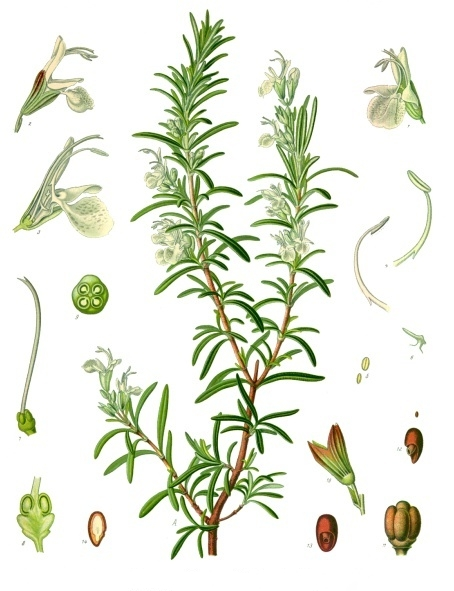
\includegraphics[width=0.5\textwidth]{romero1_hojas}
	\caption{\textit{Rosmarinus officinalis} en Kohler\'s Medicinal Plants\label{romero1_hojas}}
\end{figure}

\subsubsection{Cultivo}

Los cultivos de romero pueden realizarse por semillas o por estacas, siendo el segundo el más recomendable para realizar a grandes escalas. El cultivo por estacas consiste en cortar ramas de 0,2 metros de largo, las cuales se colocan en viveros en épocas entre otoño y primavera, se colocan en hileras distanciadas 0,2 metros y se deja un espacio de 0,15 metros entre plantas.
La densidad de la plantación es de unas 10 a 15 mil plantas por hectárea.
Una vez que las plantas emitan raíces se realiza su trasplante al campo. (cita)

Los cuidados consisten básicamente en la eliminación de malezas y, de ser necesario, recubrir con tierra. Como es una planta resistente a las sequías, los riegos deben realizarse solo en casos necesarios y en el momento del trasplante, de todas formas, estudios sugieren que el estrés por incremento del ingreso de agua a causa de precipitaciones podría promover la producción de ácido carnósico en la planta. (cita)

\begin{figure}[H]
	\centering
	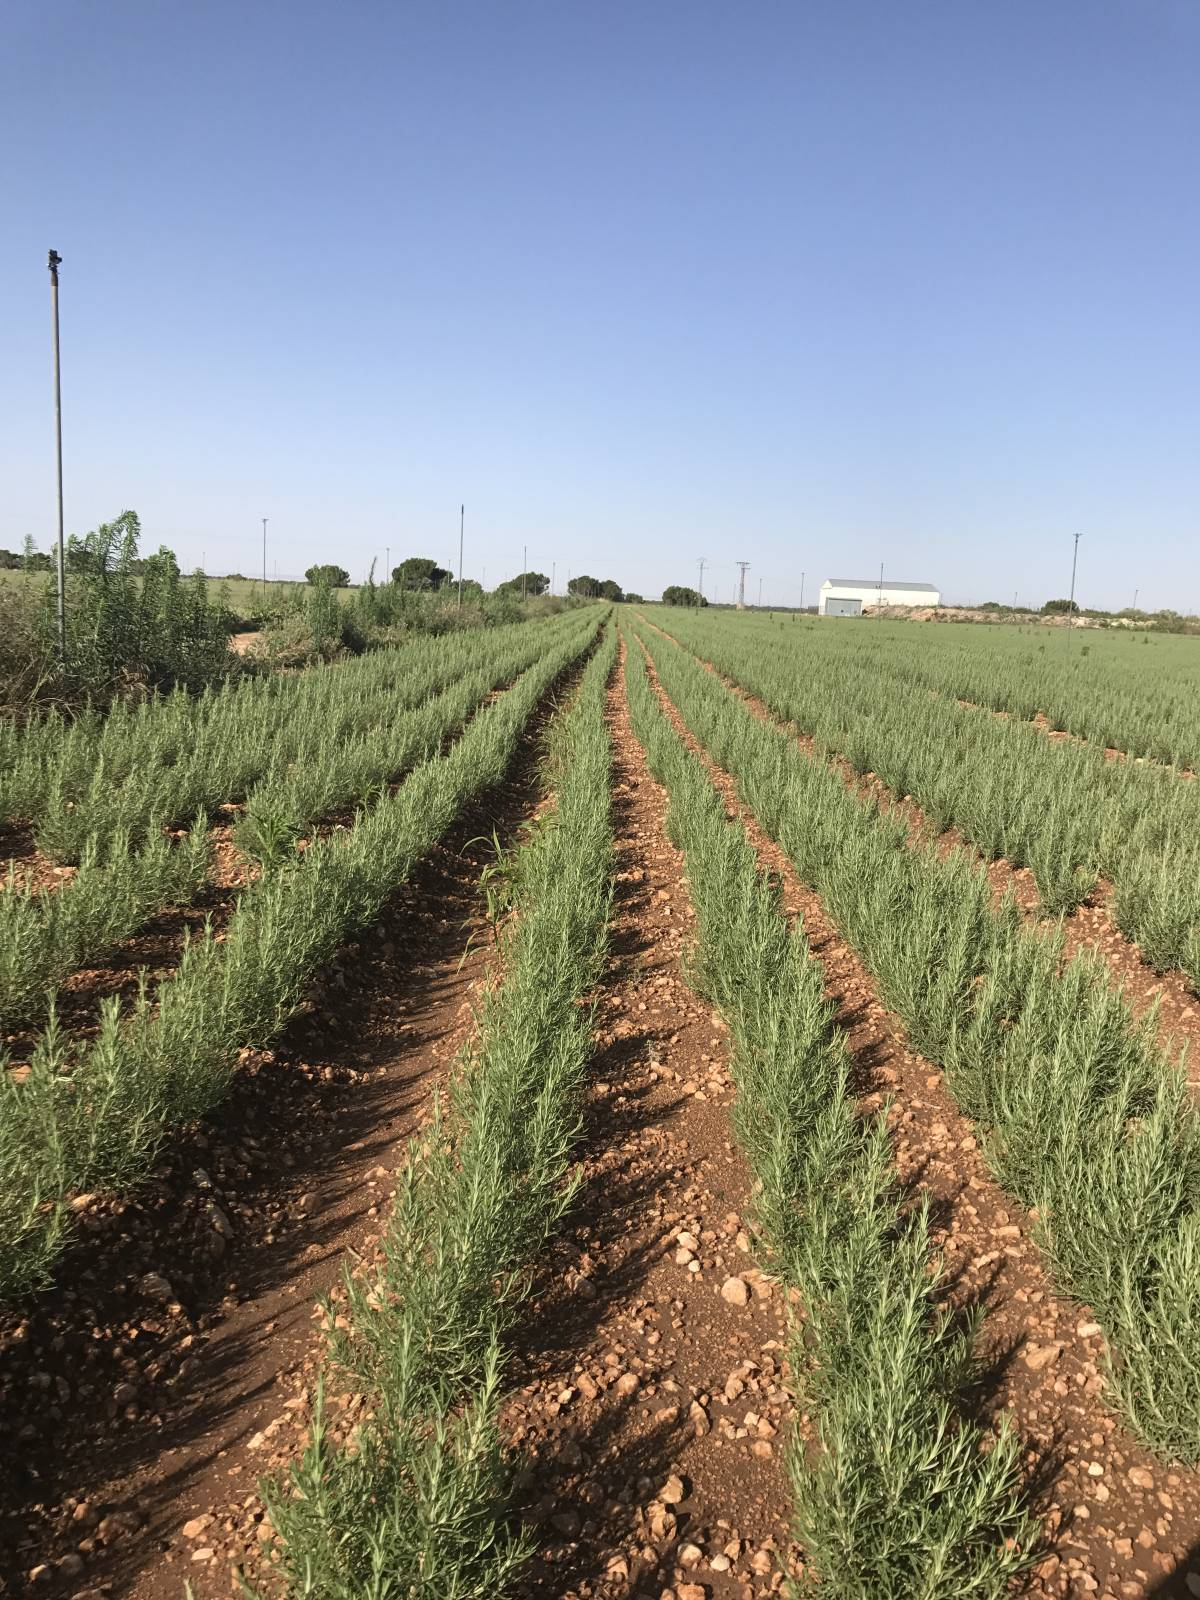
\includegraphics[width=0.5\textwidth]{romero3_plantacion}
	\caption{Plantación de romero\label{plantacion}}
\end{figure}

\subsubsection{Cosecha}

La cosecha se realiza a partir del segundo o tercer año, al comenzar la floración.
Se cortan los tallos con tijeras, favoreciendo el posterior rebrote de matas con tallos jóvenes de poca madera y abundantes hojas. La cosecha puede realizarse anualmente, aunque es preferible realizarla cada año y medio para evitar perjudicar el crecimiento de la planta.

\subsubsection{Postcosecha}

Una vez cosechadas las plantas, se realiza una operación de secado, lo normal es que se realice en bandejas, permitiendo el flujo transversal del aire por las hojas. Posteriormente se separan las hojas de los tallos, se limpian, clasifican, seleccionan y embalan. El rendimiento de producción es de entre 1200 a 1600 Kg/ha de hojas secas (cita).
Actualmente la producción de romero en el país se centra principalmente en las provincias de Córdoba y Mendoza, ocupando entre ambas 45 hectáreas de cultivos de romero (cita), esto resultaría en un estimado de producción anual de entre 36000 y 48000 Kg de hojas secas de Romero.

\subsection{Métodos Extractivos}

La extracción de productos naturales probablemente ha existido desde antes de la conformación de las primeras civilizaciones; egipcios, fenicios, judíos, árabes, indios, chinos, griegos, romanos, mayas y aztecas, todos poseían procesos innovativos de extracción, como la maceración y la destilación en alambiques, utilizados para la elaboración de perfumes, medicinas o alimentos (cita).
La maceración es una extracción sólido-líquido donde la materia prima sólida se trata con un solvente que extrae los compuestos solubles presentes en la misma, mientras que las destilaciones en alambiques consisten en tratar a la materia prima con vapor de agua, el cual arrastra los compuestos volátiles (comúnmente llamados ``aceites esenciales'' en el caso de los productos vegetales), separándolos del sólido inicial.


\subsubsection{Factores que influyen en la extracción}

\begin{descriptionB}

	\item[Propiedades de la materia prima] Las propiedades de la materia prima (humedad, porosidad, tamaño de partícula, etc.) influyen en la velocidad de extracción.
		Normalmente se parte del material molido y deshidratado para incrementar el área de contacto entre la materia vegetal y el solvente, evitando la formación de emulsiones entre el agua presente y el solvente.
		Mientras más pequeñas sean las partículas de la materia prima, mayor será el rendimiento de extracción debido a la mayor disponibilidad de los solutos gracias al fácil acceso del solvente al centro de la partícula, además, al incrementar el área de contacto entre el material y el solvente se incrementa la velocidad de extracción.

	\item[Naturaleza del solvente] La selección del solvente es fundamental en el proceso extractivo ya que de este dependerá en primera medida el rendimiento de la extracción, en función de la afinidad que tenga con el soluto a extraer.
		Las principales características a tener en cuenta al momento de seleccionar el solvente son:
		\begin{itemize}
			\item Alto límite de saturación y selectividad con respecto al compuesto a extraer.
			\item Bajo costo.
			\item Fácil de manipular y recuperar
			\item De mínimos riesgos ante una posible contaminación ambiental.
			\item Seguro de utilizar
		\end{itemize}
	\item[Agitación] La agitación es de importancia ya que favorece la velocidad de transferencia de masa desde la capa límite entre la materia vegetal y el solvente, al incrementar el valor de número de Sherwood, número adimensional que describe la relación entre la transferencia de masa de manera convectiva y la transferencia de masa de manera difusiva (Ec. \ref{Sh})
	
		\begin{equation}
			Sh = \frac{k_{c}a}{D_{12}}\label{Sh}
		\end{equation}

		Donde
		\begin{center}		

		\begin{tabular}{rlr}
			$k_{c}$ :& Coeficiente de transferencia de masa en capa límiite\\
			$a$ :& Longitud característica del sólido \\
			$D_{12}$ :& Coeficiente de difusión del soluto en el solvente \\
		\end{tabular}
		\end{center}
		El número de Sherwood aumenta con los incrementos de la velocidad de agitación, ya que es proporcional al número de Reynolds, el cual aumenta de manera lineal con respecto a la velocidad relativa entre el fluido y las partículas (Ec. \ref{Re})

		\begin{equation}
			Re = \frac{u \rho D}{\eta}\label{Re}
		\end{equation}

		Donde:
		\begin{center}	
		\begin{tabular}{ rlr}
			$u$ :	& Velocidad relativa entre sólido y líquido &$\frac{m}{s}$ \\
			$\rho$ :& Densidad del fluido  &$ \frac{Kg}{m^{3}}$ \\
		\end{tabular}
		\end{center}
	\item[Temperatura]
		La temperatura es de suma importancia en los procesos extractivos ya que, en la mayoría de los casos, incrementos de la misma causan un aumento del rendimiento de extracción como de la velocidad de la misma. En el caso de las extracciones de productos naturales es necesario tener los cuidados necesarios según el compuesto que se desea extraer, ya que estos suelen degradarse a temperaturas elevadas.

\end{descriptionB}

\subsubsection{Operaciones en batch}

Los equipamientos más comuntes para las extracciones con solventes en plantas son maceradores, los culaes consisten en tanques agitados con sistemas de control de temperatura. La maceración normalmente finaliza tras un tiempo determinado normalmente dependiente de coeficientes de partición, difusión y transferencia de masa, por lo que típicamente se realizan en etapas múltiples con el fin de alcanzar el máximo rendimiento posible, normalmente los maceradores están equipados con un doble fondo y un filtro para separar el líquido de los sólidos. \cite{Kassing 2009} (cita)

Otro método es el de percolación, el cual consiste en el flujo del solvente de extracción a través de un lecho fijo de la matriz sólida, normalmente favorecido por la gravedad. Presenta la ventaja de mantener siempre un alto gradiente de concentración debido al constante ingreso de solvente, lo cual permite un alto rendimiento de extracción.

La extracción de material botánico utilizando fluidos supercríticos es una temática de creciente interés, ya que permite el procesamiento del material a bajas temperaturas y, por lo tanto, disminuyendo la degradación térmica. La extracción utilizando gases comprimidos en condiciones críticas y cercanas a las las críticas se basa en propiedades físicas, mientras sus densidades son similares a la de los líquidos, presentas viscosidades bajas y coeficientes d edifusión altos como los gases. \cite{Kassing 2009} (cita)


\subsubsection{Procesos Continuos}

Los procesos continuos son utilizados principalmente para producción a gran escala de productos individuales. Los extractores continuos presentan dimensiones relativamente pequeñas y diseños compactos. El diseño del proceso puede diferir según el sentido del flujo de los materiales, si tanto el solvente como el material a extraer se transportan en el mismo sentido, el proceso es cocorriente, en el caso contrario se denomina contracorriente \cite{Kassing 2009} (cita)

La extracción contracorriente permite obtener productos de altas concentraciones y rendimientos gracias a que siempre mantiene un gradiente de concentración elevado entre la materia prima y el solvente, esto permite menores tiempos de extracción y productos finales de mayor calidad a comparación de los procesos batch. En la actualidad son pocas las empresas que manufacturan extractores continuos a contracorriente y la mayoría apunta a la extracción de aceite de oliva, en la tabla \ref{tipos_extractores} se pueden observar los distintos tipos de extractores realizados por estas empresas.


\begin{center}
	\includegraphics[width=1.1\textwidth]{extractors-table}
\end{center}

\begin{center}
	\begin{table}[h]
%		\small
%	\begin{tabular}{|p{1.5cm}|p{1.5cm}|p{2cm}|p{1.5cm}|p{1.5cm}|p{1.5cm}|p{1.5cm}|p{1.5cm}|}
%		\hline
%	
%		\multicolumn{3}{|p{6cm}|}{\centering Extractor} & Capacidad & Rendimiento & Relación volumétrica sólido/líquido & Tiempo de residencia (min) & Tamaño de partícula \\
%		
%		\hline
%		BMA, Alemania & MBA torre de extracción & \includegraphics[width=2cm]{bma_extractor}& 4000-17000 & 90 & 3-5 & 90-150 & 5-100
%\end{tabular}
		\caption{Extractores sólido-líquido contracorriente - Fuente:\cite{Kassing 2009}\label{tipos_extractores}}
		
	\end{table}
\end{center}




\subsubsection{Enfoques para el modelado de extracciones de plantas}

\paragraph{}
\begin{descriptionB}
\item[Modelos estadísticos mediante superficie de respuesta]
Estos modelos se utilizan especialmente para procesos de optimización de combinaciones multifactoriales, ayudando a identificar los parámetros significativos en los procesos y poder visualizar sus interacciones mutuas. En el caso de extracciones de plantas, las superficies de respuesta se utilizan para encontrar un valor óptimo de rendimiento de extracción en función de distintas variables, como temperatura, presión, relaciones masa/solvente, entre otras. Estos modelos estadísticos son capaces de describir el proceso solo en un rango predefinido de parámetros mediante el ajuste de datos experimentales y no evidencian información sobre los mecanismos de extracción del material por lo que aportan una base muy restringida pero que permite desarrollar un mejor entendimiento del proceso.

\item[Modelos rigurosos]
A diferencia de los anteriores, los modelos rigurosos son modelos matemáticos que se basan en las propiedades fisicoquímicas intrínsecas de los componentes que participan del proceso y ecuaciones diferenciales que describen el mismo, se pueden dividir en aquellos que analizan solo al nivel macroscópico (por ejemplo, al nivel del equipamiento) o aquellos que analizan al nivel microscópico (por ejemplo, al nivel de una partícula).

El equipamiento puede ser caracterizado por sus dimensiones geométricas y parámetros de proceso. Por ejemplo, para el caso de una columna, considerando dispersión axial:

\end{descriptionB}

\section{Caracterización de Materia Prima}
\subsection{Humedad\label{humedad}}
\subsection{Densidad\label{densidad}}
\subsubsection{Densidad Real}
\subsubsection{Densidad Aparente}
\subsection{Contenido de Ácido Carnósico\label{contenido_ac}}
\subsection{Distribución de tamaños de partícula}

\section{Determinación de parámetros de extracción\label{ext_param}}
\subsection{Selección de solvente\label{selec_solvent}}
\subsection{Concentraciones de equilibrio\label{equi}}
\subsection{Cinética de extracción\label{cine}}

\section{Diseño de equipo extractor}

\subsection{Modelado matemático}
\subsection{Selección de equipo de extracción}
\subsubsection{Comparación con datos experimentales}

\section{Diseño de proceso de purificación}
\subsection{Determinación de etapas de purificación}
\subsubsection{Ensayo 1:}

\section{Análisis de Costos}

\section{Conclusiones}
\pagebreak
\section{Bibliografía}
\printbibliography
\section{Anexos}


\end{document}
